\documentclass[12pt,onecolumn]{revtex4-2}
\usepackage{braket,amsmath,graphicx,setspace}
\usepackage[hidelinks]{hyperref}
\usepackage[margin=0.8in]{geometry}
\setlength{\fboxrule}{1pt}%
\setstretch{1}

\begin{document}
\title{\bf Lightning-quick introduction to single site dynamical mean field theory}
\author{Abhirup Mukherjee}
\date{Last updated: \today}
\begin{abstract}
This is a very short introduction to the philosophy and algorithm of dynamical mean field theory (DMFT). I brought these points together and wrote this up mostly to cement my own understanding of the topic. I first discuss the Curie-Weiss mean field theory in the context of the Ising model in order to provide a familiar language, and set up in a slightly different way so that it is easily generalised to DMFT. This might be useful for anyone wanting to know, in brief, what DMFT is, and how it is implemented.
\end{abstract}
\maketitle

\tableofcontents
\section{Refresher on (static) mean field theory}\label{ising_section}
The Curie-Weiss version of mean field theory involves replacing the spatial fluctuations in the Hamiltonian or the energy by an effective static field. The static field has to be determined self-consistently. To see what this means, we take the canonical example of the Ising model. Its Hamiltonian is given by
\begin{equation}\begin{aligned}
	H = J\sum_{\left<ij \right>} S_i^z S_j^z = J\sum_i S_i^z \sum_{j \in \text{NN of }i}S_j^z
\end{aligned}\end{equation}
In order to introduce the mean-field, we replace the spins \(S_j^z\) of the nearest-neighbour sites by their average value \(\left<S_j^z\right> \equiv m_j\):
\begin{equation}\begin{aligned}
	H_\text{MF} = J\sum_i S_i^z \sum_{j \in \text{NN of }i}m_j
\end{aligned}\end{equation}
Because of translation symmetry, we expect the average local magnetisation to be independent of the position \(j\): \(m_j \equiv m_\text{loc}\). If \(z\) is the coordination number of the lattice, we get
\begin{equation}\begin{aligned}
	H_\text{MF} = J\sum_i S_i^z z m = h_\text{MF} \sum_i S_i^z,
\end{aligned}\end{equation}
where we have defined the static mean field \(h_\text{MF} \equiv Jzm_\text{loc}\). This mean field Hamiltonian is solvable, in terms of \(h_\text{MF}\). The mean-field itself, however, is still unknown. To determine it, we will use the fact that if our approach is to be internally consistent, the average magnetisation \(\left<S_i^z \right>\) obtained from the mean-field Hamiltonian \(H_\text{MF}\) should be equal to that defined before, \(m_\text{loc}\). This is again demanded on grounds of translation invariance. Since \(H_\text{MF}\) just consists of decoupled spins, the local Hamiltonian has two solutions: \(S_i^z = \pm \frac{1}{2}\) with energies \(\pm \frac{h_\text{MF}}{2}\). The local partition function \(Z_\text{MF}\) and hence the magnetisation at site \(i\) is then obtained easily:
\begin{equation}\begin{aligned}
	Z_\text{MF} = 2\cosh \left(\beta h_\text{MF}/2\right), m = \frac{1}{Z_\text{MF}}\sum_{S_i^z = \pm \frac{1}{2}} S_i^z e^{-\beta h_\text{MF}S_i^z} = \tanh \left(\beta h_\text{MF}/2\right)
\end{aligned}\end{equation}
The self-consistency equation takes the form
\begin{equation}\begin{aligned}
	m_\text{loc} = m = \tanh \left(\beta Jzm_\text{loc}/2\right)
\end{aligned}\end{equation}
This equation now has to be solved numerically, to obtain the value of the local magnetisation \(m_\text{loc}\). 

Even though this approach to obtaining the local magnetisation works for the Ising model, it is not very general; for a more complicated Hamiltonian, it will not be possible to solve it analytically and obtain an explicit self-consistency equation. We will therefore re-implement mean-field theory on the Ising model but now using a different approach, one that can be generalised to other models. This new approach involves the following steps:
\begin{itemize}
	\item[1.] Assume some initial guess value of \(m_\text{loc}\).
	\item[2.] Assume the mean-field form of the Hamiltonian, \(H_\text{MF}\) in terms of the chosen \(m_\text{loc}\).
	\item[3.] Solve this Hamiltonian to obtain a local magnetisation \(m\).
	\item[4.] Take this as the updated value of \(m_\text{loc}\): \(m_\text{loc} = m\), and construct a new Hamiltonian \(H_\text{MF}\) using the updated \(m_\text{loc}\).
	\item[5.] Restart from step 3.
\end{itemize}
The idea is that we start with a guess value of the environment local magnetisation \(m_\text{loc}\) and solve the Hamiltonian with this mean-field to obtain a value for the local magnetisation, \(m\). These values will most probably not satisfy \(m = \tanh \beta J z m_\text{loc}/2\), because we guess the value of \(m_\text{loc}\). In order to get closer to the self-consistent value, we {\it update} \(m_\text{loc}\) by setting it equal to the value of \(m\) computed in the last step. We then solve the Hamiltonian with this updated value of \(m_\text{loc}\) to obtain a new value of \(m\), and these values will be closer to the self-consistent value. We keep doing this until we converge to the self-consistent value. This is shown in Fig.~\ref{ising-selfconsistency}.

\begin{figure}[htpb]
	\centering
	\fbox{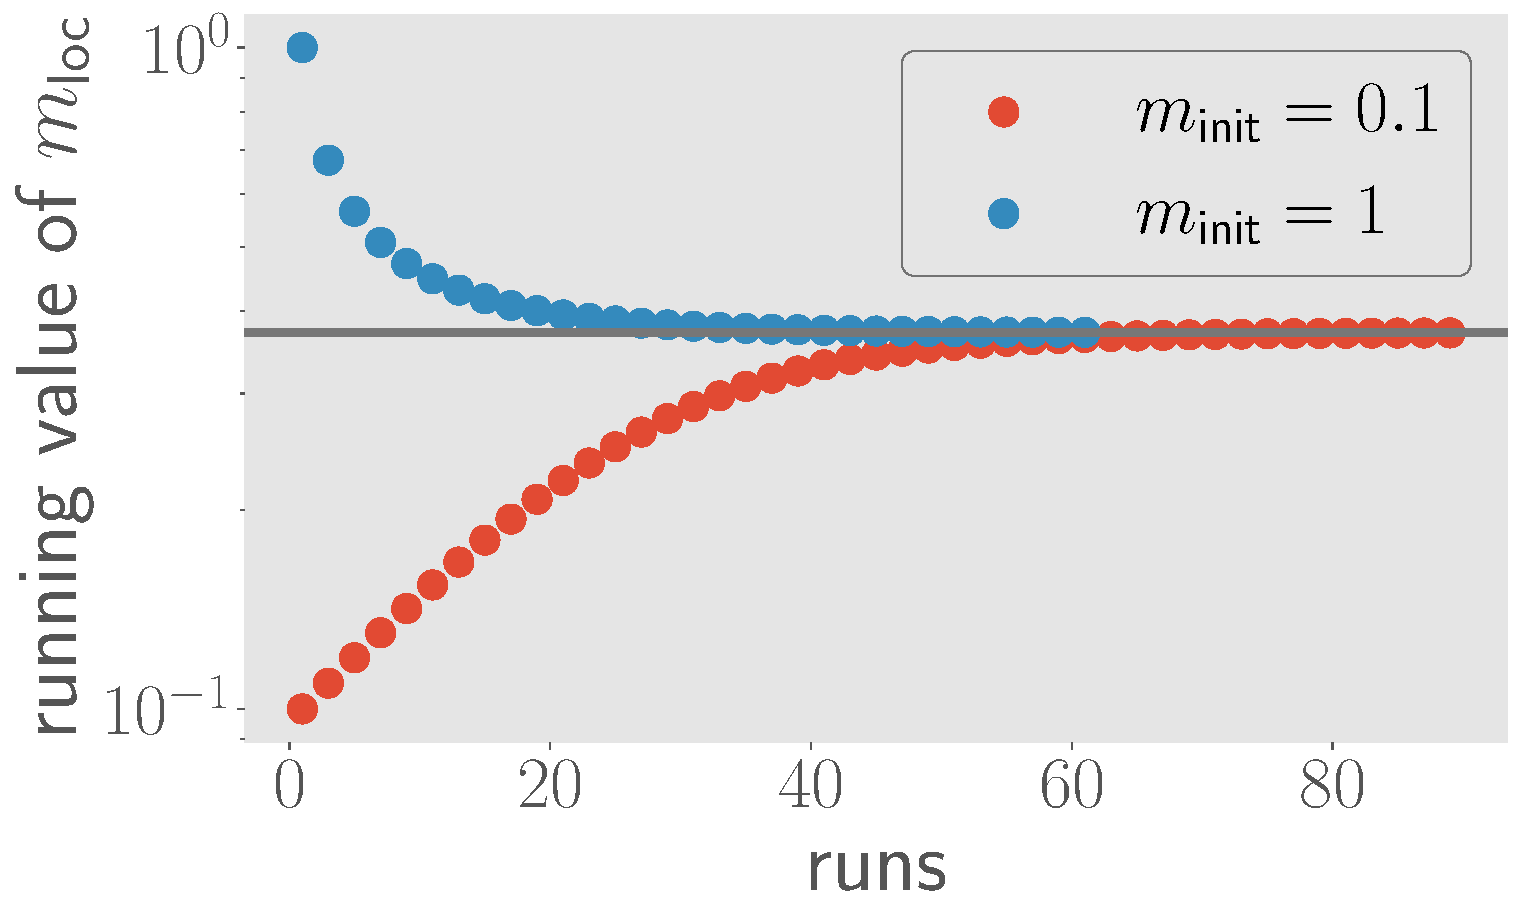
\includegraphics[width=0.6\textwidth]{ising_selfconsistency.pdf}}
	\caption{Convergence of the local magnetisation to the self-consistent value (horizontal solid line) after repeatedly solving the Hamiltonian and updating it with the solution, with \(\beta J z = 2.1\). Two examples are shown, one with the initial value \(m_\text{init}\) greater than the final value, the other less than the final value. Both converge within 90 runs.}
	\label{ising-selfconsistency}
\end{figure}

The more general approach to applying the mean field approximation can therefore be formalised as follows:
\begin{itemize}
	\item Figure out what the mean field \(y\) is. Construct a self-consistency equation out of it. It can be of the following form: $y = f(y)$, or more generally a set of coupled equations: \(y = f_1(y_1), y_1 = f_2(y_2),\ldots f_n(y_n)=y\).
	\item Replace the fluctuations by an effective local mean field \(f(y)\), in order to obtain a simpler problem (the simplified Hamiltonian \(H_\text{MF}\)).
	\item Solve the simpler problem at a particular local site \(i\) by starting with some guess value of \(f(y)\), to calculate the mean field \(y^\prime\) from it.
	\item Create an updated Hamiltonian by setting \(y=y^\prime\).
	\item Solve this new Hamiltonian to obtain yet another updated \(y^\prime\), and keep repeating this until \(y\) does not change.
\end{itemize}

\section{Dynamical mean field theory - what's the big idea?}

Dynamical mean field theory (DMFT), and mean field theory in general, falls in the class of {\it auxiliary model methods}. Such methods, very broadly, convert a bulk lattice model into the sum of a correlated impurity term and a simplified bath term that interacts with the impurity:
\begin{equation}\begin{aligned}
	\mathcal{H}_\text{full} = \sum_i \mathcal{H}_\text{loc}(i) + \sum_{\left\{ i,j,\ldots \right\}}\mathcal{H}_\text{non-loc}\left(\left\{ i,j,\ldots \right\}\right) \simeq \sum_i\left[\mathcal{H}_\text{loc}(i) + \mathcal{H}_\text{bath}(i)\right] ~.
\end{aligned}\end{equation}
The problem is then reduced to solving the impurity model \(\mathcal{H}_\text{loc}(i) + \mathcal{H}_\text{bath}(i)\). Various approximations typically go into converting the fully-interacting part \(\mathcal{H}_\text{non-loc}\left(\left\{ i,j,\ldots \right\}\right)\) into the bath Hamiltonian \(\mathcal{H}_\text{bath}(i)\), in order to make the impurity Hamiltonian tractable. In the case of the Ising model discussed in Section \ref{ising_section}, there was no purely local term in the Hamiltonian, so \(\mathcal{H}_\text{loc}(i)\) was identically zero. The non-local term was the Ising term itself: \(\mathcal{H}_\text{non-loc}\left(\left\{ i, i+1\right\}\right) = J S_i^z S_{i+1}^z\), which we simplified into \(\mathcal{H}_\text{bath}(i) = h_\text{MF} S_i^z\).

In DMFT, we cast the full interacting problem into the form of an impurity problem with a self-consistently determined bath:
\begin{equation}\begin{aligned}
	G_\text{loc} = \frac{1}{\omega - \Sigma_0 - t^2 G_\text{loc}}
\end{aligned}\end{equation}
This is the expression for the local lattice Greens function (under certain approximations which will be discussed below and which are central to the idea of DMFT), and it can be thought of as the impurity Greens function of a single impurity Anderson model. The self-consistent nature stems from the fact that the non-interacting Greens function of the impurity problem (determined by interactions with the bath) is given by \(t^2 G_\text{loc}\), where \(G_\text{loc}\) is also the final complete impurity Greens function. The problem then boils down to solving the mean field \(G_\text{loc}\) in a self-consistent fashion.

\section{Derivation of the DMFT self-consistency equation for the Hubbard model}
In DMFT, we adopt the local Greens function as our mean field. In general, the Greens function \(G_i(\omega)\) at a particular site \(i\) is a complicated object. For the case of the Hubbard model at zero chemical potential, the Hamiltonian takes the form
\begin{equation}\begin{aligned}
	\mathcal{H}_\text{HUB} = -t\sum_{\left<i,j \right>,\sigma}\left( c^\dagger_{i\sigma}c_{j\sigma} + \text{h.c.} \right) + U \sum_i \hat n_{i \uparrow} \hat n_{i \downarrow}~.
\end{aligned}\end{equation}
By identifying, say, the zeroth site of the lattice, the Hamiltonian can be formally separated into three parts:
\begin{equation}\begin{aligned}
	\mathcal{H}_\text{HUB} = \underbrace{U \sum_i \hat n_{0 \uparrow} \hat n_{0 \downarrow}}_{\mathcal{H}_0} + \underbrace{(-t)\sum_{\left<0,i \right>,\sigma}\left( c^\dagger_{i\sigma}c_{0\sigma} + \text{h.c.} \right)}_{\mathcal{H}_{0-\text{rest}}} + \underbrace{U \sum_{i \neq 0} \hat n_{i \uparrow} \hat n_{i \downarrow} -t\sum_{\left<i,j \right>\neq 0,\sigma}\left( c^\dagger_{i\sigma}c_{j\sigma} + \text{h.c.} \right)}_{\mathcal{H}_\text{rest}}~.
\end{aligned}\end{equation}
The three parts are
\begin{itemize}
	\item \(\mathcal{H}_0\): the Hamiltonian with all sites except site 0 removed,
	\item \(\mathcal{H}_\text{rest}\): the Hamiltonian with site 0 removed, and
	\item \(\mathcal{H}_{0-\text{rest}}\): the remaining part, representing the link between the first two parts. 
\end{itemize}
Let \(G\) be the real-space Greens function of the system defined by \(\mathcal{H}_\text{rest}\). The local Greens function \(G_0(\omega)\) of site 0 arising from the full Hamiltonian can be written as the sum of a ``non-interacting" part \(\mathcal{G}_0\) due to one-particle hopping into the system characterised by \(\mathcal{H}_\text{rest}\), and a self-energy arising out of the local correlation \(U\) at site 0:
\begin{equation}\begin{aligned}
	\left(1/G_0\right) = \left(1/\mathcal{G}_0\right) - \Sigma_0(\omega)~.
\end{aligned}\end{equation}
\(\mathcal{G}_0\) can be thought of as the local Greens function of the site 0 in the absence of the local correlation at that site, but in the presence of the correlation on the other sites. Calculating \(G_0^{(0)}\) is therefore is at least as hard as solving the original problem. All this is still pretty standard and exact, and no simplification has been made. We can express the Greens function \(\mathcal{G}_0\) in terms of its own self-energy \(\Sigma_\text{rest}\):
\begin{equation}\begin{aligned}
	1/\mathcal{G}_0 = \omega - \Sigma_\text{rest}
\end{aligned}\end{equation}
Note that \(\mathcal{G}_0\) represents the spectral weight of an electron hopping from the uncorrelated site 0 into the rest of the (correlated) lattice, and will therefore involve the hopping parameter \(t\) and the interacting Greens function \(G\) of \(\mathcal{H}_\text{rest}\). With this in mind, we can express the self-energy \(\Sigma_\text{rest}\) as a vertex expansion in \(G\):
\begin{equation}\begin{aligned}
	\Sigma_\text{rest} = & t^2 \sum_{\left<0,ij\right>}\int d\tau \left<\mathcal{T}_o \left(c^\dagger_{i\sigma}(\tau) c_{j\sigma}(0)\right)\right> + t^4 \sum_{\left<0,i_1j_1i_2j_2\right>}\int d\tau_1 d\tau_2 \left<\mathcal{T}_o \left(c^\dagger_{i_1\sigma}(\tau_1)c^\dagger_{i_2\sigma}(\tau_2) c_{j_1\sigma}(0)c_{j_2\sigma}(0)\right)\right>\\
			    &+ \ldots + t^{2n} \sum_{\left<0,i_1\ldots i_nj_1\ldots j_n\right>}\int d\tau_1 \ldots d\tau_n \left<\mathcal{T}_o \left(c^\dagger_{i_1\sigma}(\tau_1)\ldots c^\dagger_{i_n\sigma}(\tau_n) c_{j_1\sigma}(0)\ldots c_{j_n\sigma}(0)\right)\right> + \ldots\\
	=& t^2 \sum_{\left<0,ij \right>}\int d\tau G\left(i:j;\tau:0\right) + t^4 \sum_{\left<0,i_1j_1i_2j_2\right>}\int d\tau_1 d\tau_2 G\left(i_1,i_2:j_1,j_2;\tau_1,\tau_2:0,0\right) + \ldots \\
	 &+ t^{2n} \sum_{\left<0,i_1\ldots i_nj_1\ldots j_n\right>}\int d\tau_1 \ldots d\tau_n G\left(i_1\ldots i_n:j_1\ldots j_n;\tau_1\ldots,\tau_n:0\ldots,0\right) + \ldots~,
\end{aligned}\end{equation}
where \(\mathcal{T}_0\) is the time-ordering operator, and \(G\left(i_1\ldots i_n:j_1\ldots j_n;\tau_1\ldots,\tau_n:0\ldots,0\right)\) is the \(2n-\)point correlation function. All real-space indices \(i_1\) through \(i_n\) and \(j_1\) through \(j_n\) are summed over the real-space neighbours of \(0\). By going to frequency-domain, we get
\begin{equation}\begin{aligned}
	\Sigma_\text{rest} =& t^2 \sum_{\left<0,i_1 j_1 \right>} G_{i_1:j_1}(\omega_1) + t^4 \sum G_{i_1,i_2:j_1,j_2}(\omega_1,\omega_2) + \ldots + t^{2n} \sum G_{i_1\ldots i_n:j_1\ldots j_n}(\omega_1,\ldots \omega_n) + \ldots\label{self-energy-expansion}
\end{aligned}\end{equation}
We now introduce the first approximation. In the limit of large dimensionality \(d\), Metzner and Vollhardt have shown that the sensible way to scale the Hamiltonian is to replace \(t \to t/\sqrt{d}\). Muller-Hartmann have then showed that in the vertex expansion of Eq.\ref{self-energy-expansion}, only the purely local term \(G_{i_1;i_1}\) is of order 1, while all subsequent terms vanish at least as \(1/d\), such that they do not contribute. This simplifies the calculation enormously:
\begin{equation}\begin{aligned}
	\Sigma_\text{rest}(\omega) \simeq& \left(t^2/d\right) \sum_{\left<0,i\right>} G_{i:i}(\omega) = t^2 G_\text{loc}(\omega)
\end{aligned}\end{equation}
where we have defined \(G_\text{loc} \equiv G_{i;i}\) as the interacting local Greens function of the ``rest" system. Substituting this into \(\mathcal{G}_0\) and then into \(G_0\) gives
\begin{equation}\begin{aligned}
	G_0 = \frac{1}{\omega - t^2 G_\text{loc}(\omega) - \Sigma_0(\omega)}
\end{aligned}\end{equation}
Because of translation invariance, we expect the local Greens function of site 0 to be the same as the local Greens function of the "rest" system: \(G_0 = G_\text{loc}\), leading to a self-consistent equation in \(G_0\)
\begin{equation}\begin{aligned}
	G_0 = \frac{1}{\omega - t^2 G_0(\omega) - \Sigma_0(\omega)}~.
\end{aligned}\end{equation}
This should be recognisable as the Greens function of an Anderson impurity embedded in a conduction bath.

\section{The algorithm of the self-consistency loop}
The equations are now in place, and the only thing that is left is to solve the equation self-consistently. This is where the alternate formulation of the Ising model solution (described at the end of the first section) is useful. We will use a similar approach here to obtain the mean field in an iterative fashion. This method is often referred to as the self-consistency loop. It involves the following steps:
\begin{itemize}
	\item Create an Anderson impurity model defined by the parameters \(U\) and some initial guess of \(G_\text{loc}\). \(U\) fixes the impurity on-site correlation and \(G_\text{loc}\) sets the non-interacting local Greens function, \(\mathcal{G}^{-1} = \omega - t^2 G_\text{loc}\).
	\item Obtain the local impurity Greens function \(G_0\) using some solver like IPT, NRG, C-TQMC, etc, and hence the impurity self-energy \(\Sigma_0 = \mathcal{G}_0^{-1} - G_0^{-1}\). By self-consistency, this should also be the local self-energy of the rest of the system: \(\Sigma_0 = \Sigma_i\).
	\item As mentioned before, in infinite dimensions, all non-local contributions to the self-energy vanish, leading to a \(k-\)independent self-energy: \(\Sigma(\vec k,\omega) = \sum_{\vec r}e^{i \vec{k}\cdot\vec{r}}\Sigma(\vec r,\omega) \simeq \Sigma(\vec r=0, \omega) = \Sigma_i(\omega)\). We can therefore calculate the lattice self-energy from the impurity model solution: \(\Sigma(\vec k,\omega) = \mathcal{G}_0^{-1} - G_0^{-1}\). This is used to construct a new local lattice Greens function \(G_\text{loc} = \sum_{\vec k} G_{\vec k} = \sum_{\vec k} \left(\omega - \epsilon_{\vec k} - \Sigma(\vec k,\omega)\right)^{-1} \)
	\item Using \(U\) and the updated \(G_\text{loc}\), one can repeat all the previous steps. This is continued until the input \(G_\text{loc}\) and the output \(G_\text{loc}\) converge into each other.
\end{itemize}
The simplification of Eq.~\ref{self-energy-expansion} that removed the non-local corrections was necessary in order to reduce the problem to that of just one unknown \(G_\text{loc}\), so that just one one self-consistency equation, \(G_0 = G_\text{loc}\), would be sufficient. If not for that, there would have been more unknowns like \(G_{ij}, G_{ijkl}\) and so on, and just one equation to solve them, which is of course impossible. This simplification has the consequence that the lattice self-energy \(\Sigma(\vec k,\omega)\) has no \(k-\)dependence, a feature that holds only in infinite dimensions.

\end{document}
